% Chapter 2: Related Works
\section{Learned Gradient Compression (LGC)}

Learned Gradient Compression (LGC) \cite{Abrahamyan2022LGC} exploits gradient correlation between workers to reduce communication costs.
It splits the gradients into two parts: a common part shared across workers and an innovation component unique to each worker and its local data.
It uses a compact 1D-convolutional autoencoder on the selected top-$k$ magnitude gradients (typically $\sim0.1\%$), accumulating the rest for error feedback. The method entropy-codes the shared indices (e.g., DEFLATE) and runs one of two backends, shown in Figure~\ref{fig:lgc}:

\begin{itemize}
    \item In a parameter-server setup (PS), a shared "common" code plus an ultra-sparse per-worker "innovation" enables the server to reconstruct and average each worker's gradient.
    \item In a ring-all-reduce setup (RAR), nodes encode, average in the latent space, then decode once locally.
\end{itemize}

The autoencoder (five 1D convolution/deconvolution layers with leaky-ReLU activation) is trained after a brief warm-up ($\sim$200–300 iterations) and then applied online. Common practice is to keep the first layer uncompressed and use top-$k$ selection only on the last layer. This yields large rate reductions at near-baseline accuracy on standard CNN workloads.

From a privacy perspective, closely related learned \emph{parameter} compression shows that lossy reconstructions can both reduce communication and substantially weaken gradient-inversion attacks \cite{Chen2024ParamCompression}, suggesting LGC-style schemes may offer communication–privacy benefits in federated learning.

\begin{figure}[htbp]
    \centering
    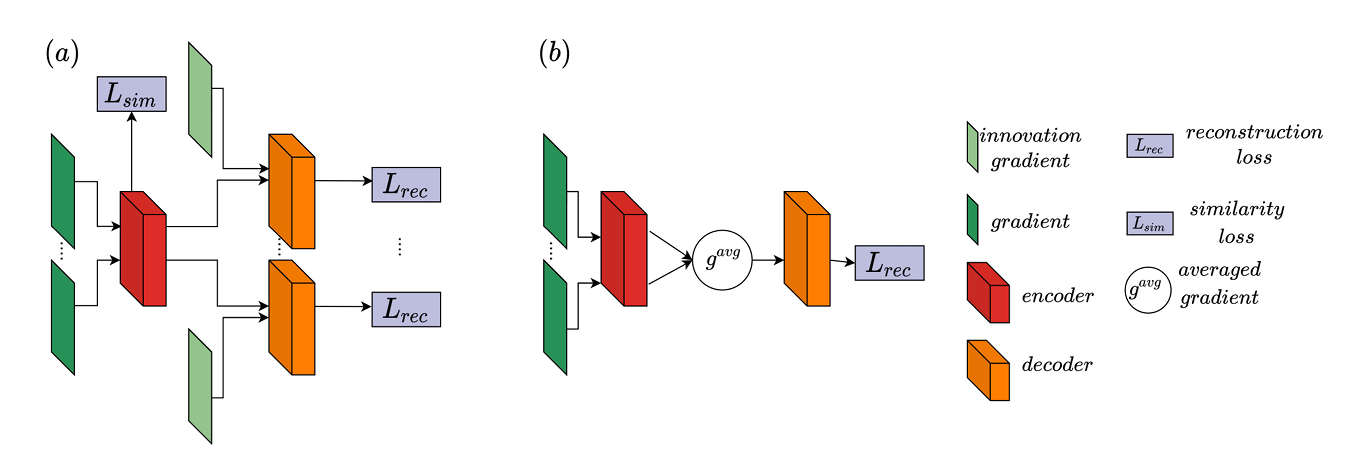
\includegraphics[width=1\textwidth]{Chapters/chapter_1_intro/figures/lgc}
    \caption{Architecture of the proposed autoencoders from \cite{Abrahamyan2022LGC} for the two different distributed communication scenarios. (a) In the PS scenario, gradients are fed sequentially to the encoder and, at each decoder, the innovation gradients are concatenated with the intermediate output before the last convolutional layer. (b) In the RAR scenario, the vectors are fed to the encoder sequentially, and after that, the outputs of the encoder form the averaged gradient, which is passed to the decoder for the reconstruction. }
    \label{fig:lgc}
\end{figure}
